\section{Widgets}
\label{ui:widgets:section:widgets}
Unter den Widgets werden in Tkinter alle grafischen Interaktionselemente wie Buttons, Labels,
Listboxes sowie Canvas etc. verstanden. Tkinter bietet hierf�r bereits vorgefertigte Klassen,
aus denen diese Widgets erzeugt werden k�nnen. Im Rahmen dieses Kapitels wird eine
Anwendung erstellt, die den Umgang mit einigen Widgets verdeutlichen soll und fortlaufend
dahingehend erweitert wird.

\subsection{Frame}
\label{ui:widgets:subsection:frame}
Frames fungieren, �hnlich wie die sogenannten divs in HTML, als Container um verschiedene
Widgets oder weitere Frames in einem bestimmten Bereich des Fensters zu gruppieren.
Dabei wird ein Rechteck erstellt und dem Eltern-Element �ber den Layout-Manager hinzugef�gt.
In folgendem Beispiel werden drei Frames erzeugt, die sich untereinander befinden und
unterschiedliche Hintergrundfarben besitzen. Um zu verdeutlichen, dass weitere Widgets
jetzt den jeweiligen Frame-Bereichen zugeordnet werden k�nnen, wird in jedem Frame ein
Label hinzugef�gt. Somit kann die Platzierung von Widgets besser kontrolliert werden.

\lstinputlisting[language=Python]{chapters/userInterface/src/GUI_FrameExample.py}
\label{ui:widgets:lst:lstinputlisting:gui_frameExample}

\begin{figure}[ht]
	\centering
	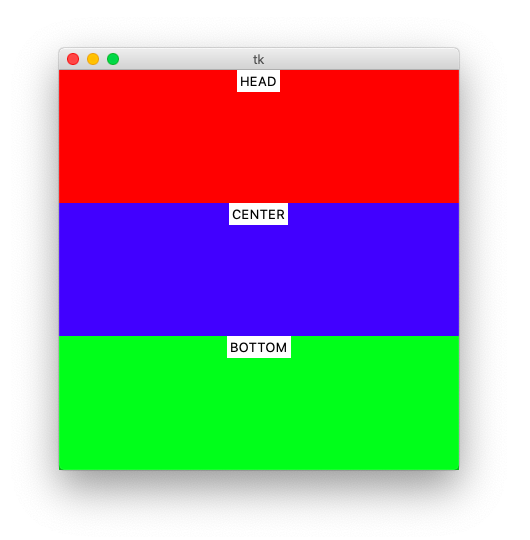
\includegraphics[width=0.5\textwidth]{images/FrameExampleGUI.png}
	\caption{Frame-Widget Beispiel}
	\label{ui:layoutManager:img:FrameExampleGUI}
\end{figure}

\subsection{Label}
\label{ui:widgets:subsection:label}
�ber Labels k�nnen im Userinterface einfache Textzeilen ausgegeben werden.
Diese lassen sich weiterhin auch dynamisch ver�ndern (z.B. bei einem Klick auf einen Button).

\subsection{Button}
\label{ui:widgets:subsection:button}
Mit dem Button hat der Nutzer die M�glichkeit mit dem Userinterface �ber einen Maus-Klick
zu interagieren. Buttons werden aus der Klasse \lstinline$Button$ erzeugt, dem Fenster oder Frame
bekannt gemacht und mit einem Text versehen. Zus�tzlich kann dem Button �ber \lstinline$command$
noch eine Funktion zugewiesen werden, die ausgef�hrt wird, sobald der Button gedr�ckt wurde.
In folgendem Beispiel wird bei Dr�cken des Buttons, in einem Label der Satz \lstinline$Hallo Python-World$
ausgegeben.

\lstinputlisting[language=Python]{chapters/userInterface/src/GUI_ButtonLabelExample.py}
\label{ui:widgets:lst:lstinputlisting:gui_buttonLabelExample}

\begin{figure}[ht]
	\centering
	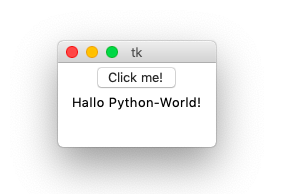
\includegraphics[width=0.5\textwidth]{images/ButtonLabelGUI.png}
	\caption{Button- und Label-Widget Beispiel}
	\label{ui:layoutManager:img:ButtonLabelGUI}
\end{figure}

\subsection{Entry}
\label{ui:widgets:subsection:entry}
�ber die sogenannten Entries lassen sich Eingaben vom Nutzer erfassen. Diese k�nnen dann im
Python-Skript weiterverarbeitet werden. Das vorherige Beispiel wird nun dementsprechend
erweitert, dass der Text, der bei Klick auf den Button ausgegeben wird, �ber \lstinline$get()$
vom Entry entgegen genommen wird.

\lstinputlisting[language=Python]{chapters/userInterface/src/GUI_EntryExample.py}
\label{ui:widgets:lst:lstinputlisting:gui_buttonLabelExample}

\begin{figure}[ht]
	\centering
	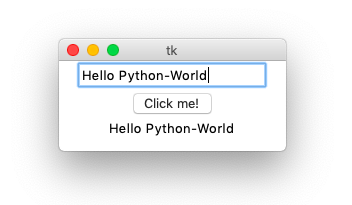
\includegraphics[width=0.5\textwidth]{images/EntryExampleGUI.png}
	\caption{Entry-Widget Beispiel}
	\label{ui:layoutManager:img:EntryExampleGUI}
\end{figure}

\subsection{Listbox}
\label{ui:widgets:subsection:listbox}
Um verschiedene Elemente in einer Liste anzeigen zu k�nnen bietet sich die Listbox an.
Der Text der vom Entry entgegengenommen wird soll nun einer solchen Listbox hinzugef�gt werden.
Dazu dient die Funktion \lstinline$insert()$. Der erste Parameter der �bergeben wird bestimmt
die Position in der Liste und der zweite das eigentliche Element.
Zus�tzlich wird der Anwendung ein zweiter Button hinzugef�gt um das jeweilig angew�hlte Element
der Listbox zu entfernen. Die Funktion \lstinline$curselection()$ gibt eine Liste der angew�hlten
Elemente zur�ck. Mithilfe von \lstinline$delete()$ wird dann das erste Element der zur�ckgegebenen Liste
aus der Listbox entfernt.

\lstinputlisting[language=Python]{chapters/userInterface/src/GUI_ListboxExample.py}
\label{ui:widgets:lst:lstinputlisting:gui_listboxwExample}

\begin{figure}[ht]
	\centering
	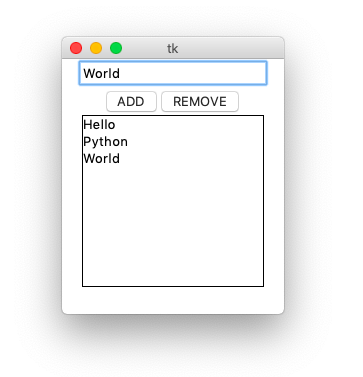
\includegraphics[width=0.5\textwidth]{images/ListboxExampleGUI.png}
	\caption{Listbox-Widget Beispiel}
	\label{ui:layoutManager:img:ListboxExampleGUI}
\end{figure}

%\subsection{Colorpicker}
%\label{ui:widgets:subsection:colorpicker}

%\subsection{Canvas}
%\label{ui:widgets:subsection:canvas}

\uebung
\aufgabe{UI_aufgabe03}
\aufgabe{UI_aufgabe04}
\aufgabe{UI_aufgabe05}
\aufgabe{UI_aufgabe06}
\aufgabe{UI_aufgabe07}
\aufgabe{UI_aufgabe08}
\aufgabe{UI_aufgabe09}
